% Kaelix — análise por simulação computacional
% Compilar:  latexmk -pdf relatorio-kaelix.tex   (ou pdflatex duas vezes)

\documentclass[10pt,a4paper,landscape,twocolumn]{article}

\usepackage[T1]{fontenc}
\usepackage[utf8]{inputenc}
\usepackage[brazil]{babel}
\usepackage{lmodern}
\usepackage[landscape,top=1.8cm,bottom=1.8cm,left=2cm,right=2cm]{geometry}
% Duas colunas em paisagem: cada uma com ~12,3 cm. O vão precisa ser
% generoso porque a linha é curta e colunas coladas cansam.
\setlength{\columnsep}{8mm}

% Floats que ocupam as duas colunas: o default (dbltopfraction 0,7) manda
% para página própria qualquer figura grande, e o resultado é página de
% float com três linhas de texto. Estes valores deixam figura e texto
% dividirem a página.
\renewcommand{\dbltopfraction}{0.92}
\renewcommand{\dblfloatpagefraction}{0.88}
\setcounter{dbltopnumber}{2}
\usepackage{booktabs}
\usepackage{siunitx}
\usepackage{graphicx}
\usepackage{amsmath}
\usepackage{amssymb}
\usepackage{microtype}
\usepackage[hidelinks]{hyperref}
\usepackage{caption}
\usepackage{enumitem}
\usepackage{xcolor}
\usepackage{titlesec}
\usepackage{float}

% Floats: permitir mais figura por página e evitar páginas de float esvaziadas
\setcounter{topnumber}{2}
\setcounter{bottomnumber}{2}
\setcounter{totalnumber}{4}
\renewcommand{\topfraction}{0.92}
\renewcommand{\bottomfraction}{0.75}
\renewcommand{\textfraction}{0.04}
\renewcommand{\floatpagefraction}{0.92}

% Figuras largas: avançam levemente sobre as margens para preservar legibilidade
\newcommand{\figuralarga}[1]{%
  \makebox[\textwidth][c]{\includegraphics[width=1.13\textwidth]{#1}}}

\sisetup{output-decimal-marker={,}, group-separator={.}, per-mode=symbol}
\captionsetup{font=footnotesize, labelfont=bf, width=0.94\textwidth}
\setlist{itemsep=2pt, topsep=4pt, parsep=0pt}
\titleformat{\section}{\normalfont\large\bfseries}{\thesection}{0.7em}{}
\titleformat{\subsection}{\normalfont\normalsize\bfseries}{\thesubsection}{0.7em}{}
\graphicspath{{../../experiments/figures/output/}{../img/}}

\newcommand{\pt}{\,p.p.}

\begin{document}

\twocolumn[{%
\noindent
\begin{minipage}[c]{0.10\textwidth}
  
\includegraphics[width=\linewidth]{skala_logo.jpeg}
\end{minipage}%
\begin{minipage}[c]{0.90\textwidth}
  \centering
  {\LARGE\bfseries Kaelix: comunicação e topologia}\\[4pt]
  {\large Comparação com dispositivos publicados, arquitetura de rede
  e cadeia de dados do sensor ao manutentor}\\[8pt]
  {\normalsize setembro de 2026}
\end{minipage}

\vspace{6pt}
\hrule
\vspace{14pt}
}]

\section{Escopo}

Este documento trata do transporte e do consumo dos dados do Kaelix: o que o dispositivo
transmite, por qual enlace, para qual receptor, e como isso se compara ao que está
publicado. Nenhum número vem de medição em hardware --- os do Kaelix saem de cálculo sobre a configuração implementada, e
os dos sistemas comparados, de folha de dados ou artigo conferido em fonte primária.

\section{Comparação com dispositivos publicados}

\subsection{Banda de aquisição}

A banda de aquisição é a principal diferença entre o Kaelix e os produtos comerciais.
Com amostragem de \SI{1}{\kilo\hertz} no MPU6050, a frequência de Nyquist fica
em \SI{500}{\hertz}. O Ranger Pro cobre \SIrange{5}{10000}{\hertz} no eixo
Z~\cite{bentlynevada2025}; no Phantom, mesmo a variante de alta sensibilidade EPH-V10E
alcança \SIrange{0,5}{4}{\kilo\hertz} em X e Y~\cite{erbessd2025}. Os três produtos
comerciais medem, em ao menos um eixo, uma ordem de grandeza acima do teto do
MPU6050~\cite{bentlynevada2025,erbessd2025,tractian2022}.

Isso delimita as falhas detectáveis: a assinatura de defeito incipiente de rolamento reside
em ressonâncias de alta frequência, fora da banda disponível~\cite{landi2023}, enquanto
desbalanceamento e desalinhamento, em múltiplos da rotação, estão dentro dela.

\subsection{Fonte de energia}

O Kaelix adota bateria recarregável com recarga por USB-C, e nenhum sistema revisado faz
isso. O circuito de carga existe a partir da placa v3, com carregador linear que suspende
a carga fora da faixa de \SIrange{0}{45}{\celsius}; até a v2 a placa não tinha como
carregar a célula. Os sistemas revisados usam célula primária: LiSOCl$_2$ de até cinco
anos no Ranger Pro~\cite{bentlynevada2025}, CR2477 para cerca de \num{65000} medições no
Phantom~\cite{erbessd2025}, lítio não substituível no Smart Trac~\cite{tractian2022}. A
temperatura ambiente admissível do Ranger Pro é fixada \emph{pela célula}, não
pelo invólucro --- o mesmo tipo de limite identificado na análise térmica do
Kaelix~\cite{bentlynevada2025}.

\subsection{Detector embarcado}

O trabalho mais próximo em arquitetura treina e executa Isolation Forest no
ESP32, em MicroPython, com IMU a \SI{1125}{\hertz}~\cite{antonini2023}. Ele fixa o escore
normalizado em \num{0,75} e declara que avaliar a acurácia de detecção está fora de
escopo. Bisio \emph{et al.} descrevem nó IIoT de vibração com a mesma classe de
hardware~\cite{bisio2025}. O nó de Kolok \emph{et al.}, também ESP32 com MPU6050, reporta
ROC-AUC de \num{0,780} e validação cruzada de cinco dobras em \SI{72,9}{\percent}
$\pm$~\SI{2,4}{\percent}, sobre cerca de \num{900} amostras e \emph{um único} modo de
falha, com rolamento adiado para trabalho futuro~\cite{kolok2025}.

\begin{table*}[!t]
\centering
\caption{Kaelix e sistemas comparáveis. Valores de banda e energia vêm de folha de dados
ou artigo; os do Kaelix, de cálculo sobre a configuração implementada.}
\footnotesize
\begin{tabular}{@{}lllll@{}}
\toprule
 & Banda & Energia & Detector & Protocolo de avaliação \\
\midrule
Ranger Pro & \SIrange{5}{10000}{\hertz} (Z) & LiSOCl$_2$, 5 anos & --- & --- \\
Phantom Gen 3 & \SIrange{0,5}{4}{\kilo\hertz} (X/Y) & CR2477 & --- & --- \\
Smart Trac & --- & lítio fixo & --- & --- \\
Antonini \emph{et al.} & \SI{1125}{\hertz} & --- & iForest \emph{on-device} & acurácia fora de escopo \\
Kolok \emph{et al.} & \SI{1}{\kilo\hertz} interno & --- & iForest & 5 dobras, 1 modo de falha \\
\textbf{Kaelix} & \SIrange{10}{500}{\hertz} & LiPo recarregável & iForest nativo em C++ & \textit{GroupKFold} por ensaio \\
\bottomrule
\end{tabular}
\end{table*}

\section{Topologia de rede}

Quatro arranjos foram comparados (Fig.~\ref{fig:topo}). Três diferem apenas no elemento
receptor --- gateway ESP32 de canal único, computador de placa única ou concentrador
LoRaWAN --- e a escolha entre eles é de escopo, não de viabilidade.

\begin{figure*}[!t]
\centering
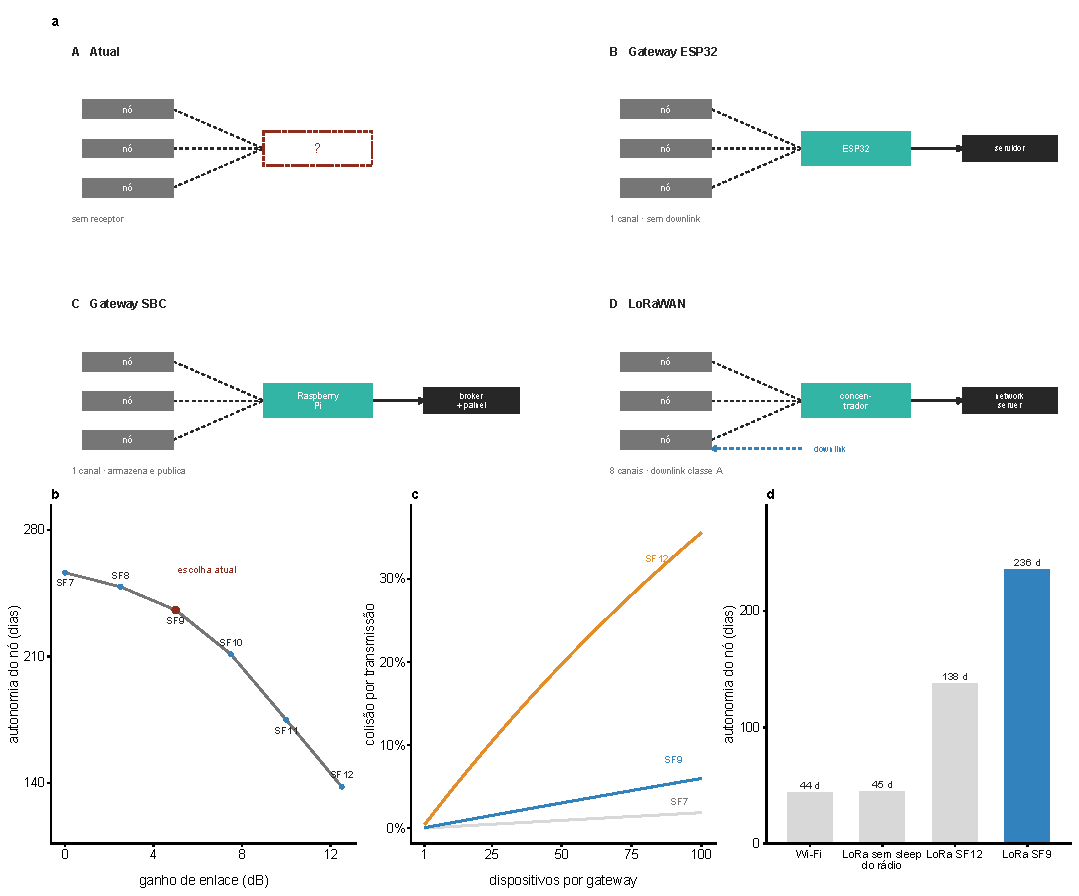
\includegraphics[width=0.62\textwidth]{fig5_topologia}
\caption{Arquiteturas topológicas comparadas. \textbf{a}, os quatro arranjos; A é o estado
anterior a este trabalho, sem receptor. \textbf{b}, autonomia contra ganho de enlace por
fator de espalhamento. \textbf{c}, colisão em ALOHA puro contra número de
dispositivos. \textbf{d}, autonomia por tecnologia de enlace.}
\label{fig:topo}
\end{figure*}

\subsection{Parâmetros do enlace e compromisso alcance--autonomia}

Os parâmetros do enlace foram fixados explicitamente em SF9, \SI{125}{\kilo\hertz} e taxa
de codificação 4/5. Antes herdavam o padrão da biblioteca, de modo que uma atualização
alteraria o consumo do produto sem que a mudança fosse detectável. O tempo no ar resultante é de
\SI{185}{\milli\second}, contra os \SI{150}{\milli\second} que o orçamento anterior
assumia sem derivação. A escolha custa autonomia --- \SI{256}{\day} em SF7 contra
\SI{138}{\day} em SF12, com \SI{12,5}{\decibel} de ganho entre os extremos --- e a
decisão definitiva depende da distância até o gateway, ainda não medida.

\subsection{Comparação com Wi-Fi}

Com associação e transmissão modeladas em \SI{5}{\second} a \SI{150}{\milli\ampere}, a
autonomia cai para \SI{44}{\day}, contra \SI{236}{\day} em LoRa SF9. O valor é próximo ao
obtido quando o SX1278 não é colocado em \emph{sleep}: o rádio permanece em
\emph{standby} durante o repouso e a autonomia fica em \SI{45}{\day}. Manter o rádio em
\emph{standby} tem custo energético equivalente ao de adotar Wi-Fi.

\section{Cadeia de dados e gateway}

A cadeia vai do motor ao manutentor em dez elos (Fig.~\ref{fig:cadeia}). Até este
trabalho os quatro últimos não existiam: o dispositivo transmitia sem receptor, e o formato do
pacote fora definido sem contraparte.

\begin{figure*}[!t]
\centering
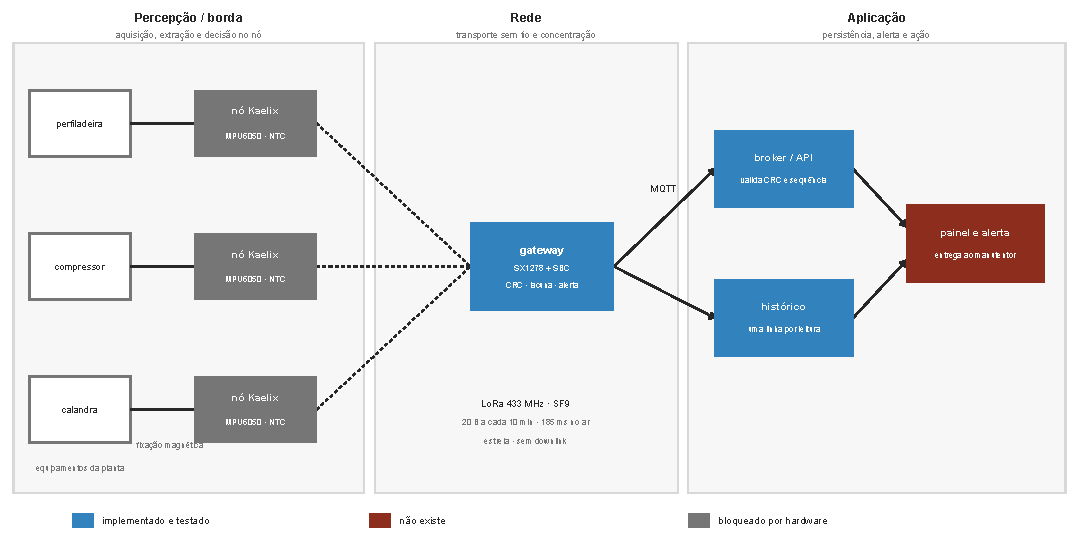
\includegraphics[width=0.71\textwidth]{fig6_cadeia}
\caption{Cadeia do sistema e estado de implementação de cada elo. Linhas tracejadas
verticais marcam a fronteira do ESP32-S3, que não coincide com a quebra de linha.
``Testado'' refere-se a verificação no \emph{host}: nenhum elo foi exercitado com rádio ou
sensor reais.}
\label{fig:cadeia}
\end{figure*}

\subsection{Funções do receptor}

O receptor assume três responsabilidades que o dispositivo não pode ter: carimbar o tempo,
já que o contador de partida dá ordem e não instante; detectar lacuna na sequência, porque
perda silenciosa é indistinguível de máquina parada; e decidir quando abrir alerta. A
regra de disparo é implementada no gateway porque alterá-la no dispositivo exigiria
regravar cada aparelho. A verificação de integridade é a mesma dos dois lados: o CRC-16 do
gateway é comparado contra o do firmware compilado com \texttt{g++}, em \num{204} casos.

\subsection{Simulação do enlace}

Sem hardware, a cadeia foi exercitada injetando os efeitos que o meio impõe: colisão,
perda e corrupção de bit (Fig.~\ref{fig:gw}). O que a simulação \emph{não} cobre é
propagação --- alcance e margem de enlace dependem de medição em campo.

\begin{figure*}[!t]
\centering
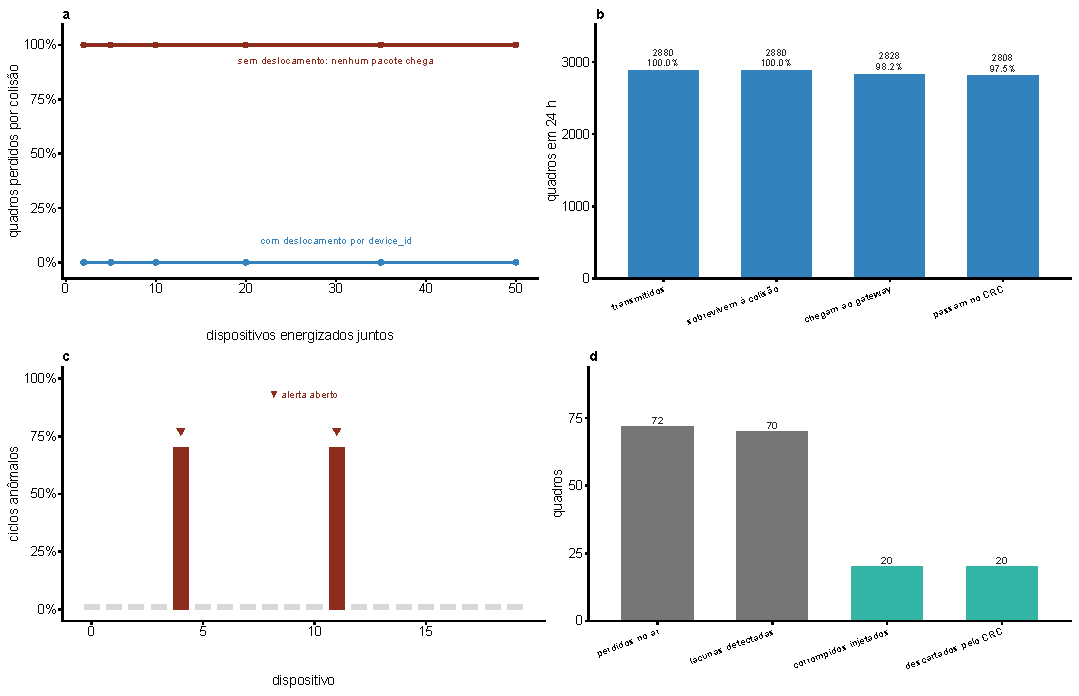
\includegraphics[width=0.66\textwidth]{fig7_gateway}
\caption{Cadeia de comunicação sob simulação de meio. \textbf{a}, colisão contra número de
dispositivos energizados simultaneamente. \textbf{b}, funil de \SI{24}{\hour} para
\num{20} dispositivos. \textbf{c}, alerta por dispositivo. \textbf{d}, perda e corrupção
injetadas no meio contra o detectado pelo gateway.}
\label{fig:gw}
\end{figure*}

O cálculo de colisão em ALOHA puro pressupõe fases de transmissão descorrelacionadas, e
uma instalação cujos aparelhos são energizados juntos não satisfaz essa hipótese: eles
transmitem no mesmo instante a cada ciclo, e a colisão é sistemática em vez de
probabilística. Sem o deslocamento derivado do identificador de dispositivo, nenhum quadro
é entregue, para qualquer número de nós; com ele, a colisão medida é nula no mesmo
cenário.

Em campanha de \SI{24}{\hour} com \num{20} dispositivos, \SI{2}{\percent} de perda e
\SI{1}{\percent} de corrupção injetados, \SI{97,5}{\percent} dos quadros viraram leitura
válida, os \num{20} corrompidos foram integralmente detectados pelo CRC, e o alerta abriu
nos dois dispositivos com anomalia sustentada e em nenhum dos dezoito com anomalia
esporádica.

\footnotesize
\begin{thebibliography}{99}
\setlength{\itemsep}{2pt}

\bibitem{antonini2023}
M.~Antonini, M.~Pincheira, M.~Vecchio e F.~Antonelli,
\newblock An adaptable and unsupervised TinyML anomaly detection system for extreme industrial environments,
\newblock \emph{Sensors}, v.~23, n.~4, art.~2344, 2023.
\newblock DOI: 10.3390/s23042344.

\bibitem{bentlynevada2025}
Bently Nevada (Baker Hughes),
\newblock \emph{Ranger Pro wireless condition monitoring} --- folha de dados, doc.\ 125M5237 Rev.~U,
\newblock Baker Hughes, 16 jul.\ 2025. Revisão corrente Rev.~V (dez.\ 2025), com valores técnicos idênticos.
\newblock Literatura de fabricante, não revisada por pares.

\bibitem{bisio2025}
I.~Bisio, C.~Garibotto, A.~Grattarola, A.~Iscra, F.~Lavagetto, A.~Sciarrone e M.~Zerbino,
\newblock Design, implementation and performance of an IIoT node for vibration monitoring,
\newblock \emph{2025 IEEE International Symposium on Circuits and Systems (ISCAS)}, Londres, p.~1--4, 2025.
\newblock DOI: 10.1109/ISCAS56072.2025.11043851.
\newblock Texto integral não acessado (assinatura); citado apenas como contexto.

\bibitem{erbessd2025}
Erbessd Instruments,
\newblock \emph{PHANTOM Gen~3 vibration sensor} --- folha de dados (EPH-V10E / EPH-V11E), rev.\ 11/2025,
\newblock Erbessd Instruments, 2025.
\newblock Literatura de fabricante, não revisada por pares.

\bibitem{kolok2025}
P.~Kolok, M.~Hodoň, P.~Ševčík, L.~Hotz e N.~Remy,
\newblock Low-cost IoT-based predictive maintenance using vibration,
\newblock \emph{Sensors}, v.~25, n.~21, art.~6610, 2025.
\newblock DOI: 10.3390/s25216610.
\newblock O artigo é internamente inconsistente: a discussão menciona \SI{93,4}{\percent} de acurácia, número ausente dos resultados; adota-se aqui apenas \SI{72,9}{\percent} (Tabela~3).

\bibitem{landi2023}
E.~Landi, A.~Prato, A.~Fort, M.~Mugnaini, V.~Vignoli, A.~Facello, F.~Mazzoleni, M.~Murgia e A.~Schiavi,
\newblock Highly reliable multicomponent MEMS sensor for predictive maintenance management of rolling bearings,
\newblock \emph{Micromachines}, v.~14, n.~2, art.~376, 2023.
\newblock DOI: 10.3390/mi14020376.

\bibitem{tractian2022}
TRACTIAN,
\newblock \emph{Smart Trac --- automated machine monitoring} --- folha de dados,
\newblock TRACTIAN, São Paulo, ago.\ 2022.
\newblock Literatura de fabricante, não revisada por pares.

\end{thebibliography}

\end{document}
